\documentclass[tikz, border=8pt]{standalone}
\usepackage{tikz}
\usetikzlibrary{calc}
\definecolor{navy}{HTML}{14213D}
\definecolor{teal}{HTML}{0E7C7B}
\definecolor{emas}{HTML}{C9A227}
\definecolor{abu}{HTML}{E8E8E8}

% Garis tinggi segitiga tumpul: dua dari tiga garis tinggi jatuh
% di luar segitiga, sehingga alas (atau sisinya) harus diperpanjang.
%
% Segitiga: A = (0,0), B = (5,0), C = (6.5,3).
% Sudut di B tumpul, sekitar 116,6 derajat.
% Kaki tinggi dari C: D = (6,5, 0), di luar segitiga (di kanan B).
% Kaki tinggi dari A: E = (4, -2), di luar segitiga (di bawah alas).
% Kaki tinggi dari B: F = (4,12, 1,90), di dalam ruas AC.
% Titik tinggi (ortosentrum): H = (6,5, -3,25), di luar segitiga.
% Luas dari ketiga pasangan alas-tinggi sama: 7,5 cm^2.
%
% Gambar 1: segitiga + garis tinggi dari C saja (alas diperpanjang).
% Gambar 2: ketiga garis tinggi + titik tinggi H.

\begin{document}

% ---------------- Gambar 1: garis tinggi dari C ----------------
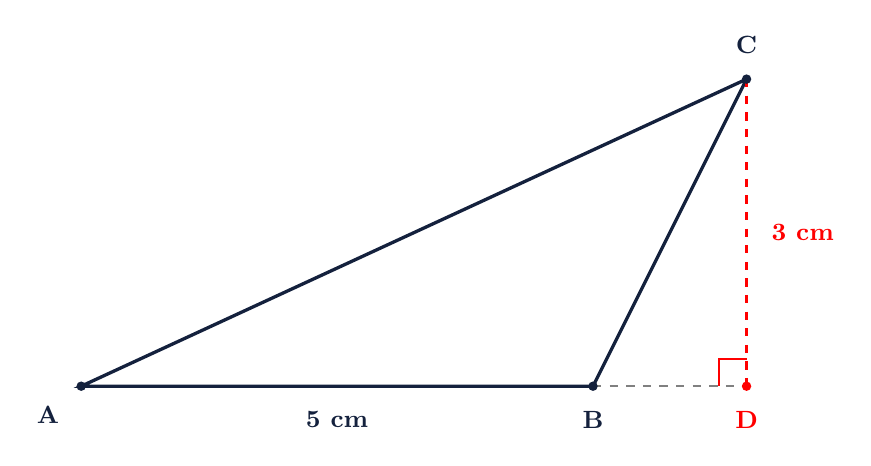
\begin{tikzpicture}[x=1.3cm, y=1.3cm]
  \coordinate (A) at (0,0);
  \coordinate (B) at (5,0);
  \coordinate (C) at (6.5,3);
  \coordinate (D) at (6.5,0); % kaki tinggi dari C, di luar segitiga
  % Sisi segitiga
  \draw[navy, very thick] (A) -- (B) -- (C) -- cycle;
  % Perpanjangan alas melewati B sampai D
  \draw[gray, thick, dashed] (B) -- (D);
  % Garis tinggi dari C, CD = 3 cm
  \draw[red, thick, dashed] (C) -- (D);
  % Tanda siku di D (pola calc: berlaku di kaki mana pun)
  \draw[red, thick] ($(D)!0.35cm!(C)$)
    -- ($($(D)!0.35cm!(C)$) + ($(D)!0.35cm!(B)$) - (D)$)
    -- ($(D)!0.35cm!(B)$);
  % Titik sudut dan kaki tinggi
  \fill[navy] (A) circle (0.06cm);
  \fill[navy] (B) circle (0.06cm);
  \fill[navy] (C) circle (0.06cm);
  \fill[red] (D) circle (0.06cm);
  \node[anchor=north east, font=\small\bfseries, navy] at (-0.12,-0.1) {A};
  \node[anchor=north, font=\small\bfseries, navy] at (5,-0.15) {B};
  \node[anchor=south, font=\small\bfseries, navy] at (6.5,3.15) {C};
  \node[anchor=north, font=\small\bfseries, red] at (6.5,-0.15) {D};
  \node[anchor=north, font=\small\bfseries, navy] at (2.5,-0.15) {5 cm};
  \node[anchor=west, font=\small\bfseries, red] at (6.65,1.5) {3 cm};
\end{tikzpicture}

% ---------------- Gambar 2: ketiga garis tinggi ----------------
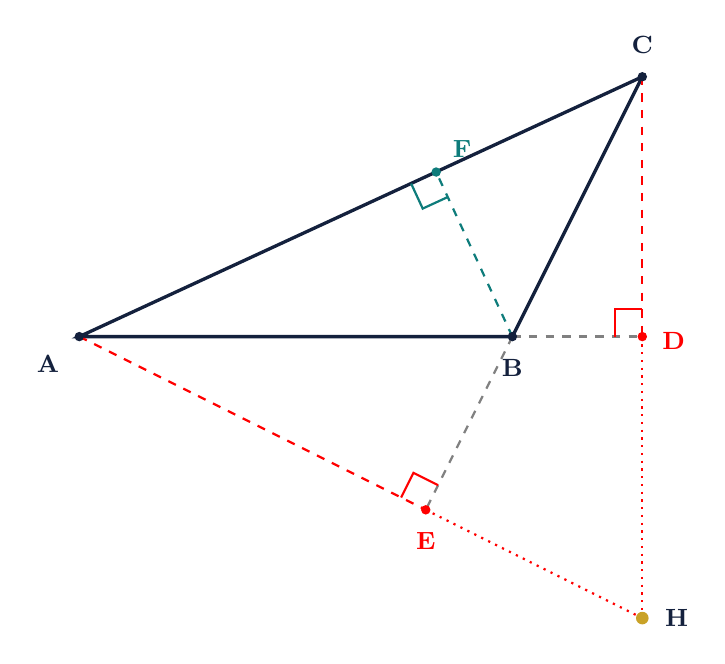
\begin{tikzpicture}[x=1.1cm, y=1.1cm]
  \coordinate (A) at (0,0);
  \coordinate (B) at (5,0);
  \coordinate (C) at (6.5,3);
  \coordinate (D) at (6.5,0);   % kaki tinggi dari C
  \coordinate (E) at (4,-2);    % kaki tinggi dari A
  \coordinate (F) at (4.12,1.90); % kaki tinggi dari B
  \coordinate (H) at (6.5,-3.25); % titik tinggi (ortosentrum)
  % Sisi segitiga
  \draw[navy, very thick] (A) -- (B) -- (C) -- cycle;
  % Perpanjangan sisi: alas melewati B ke D, sisi BC melewati B ke E
  \draw[gray, thick, dashed] (B) -- (D);
  \draw[gray, thick, dashed] (B) -- (E);
  % Ketiga garis tinggi
  \draw[red, thick, dashed] (C) -- (D);
  \draw[red, thick, dashed] (A) -- (E);
  \draw[teal, thick, dashed] (B) -- (F);
  % Perpanjangan garis tinggi dari C dan A sampai titik tinggi H
  \draw[red, thick, dotted] (D) -- (H);
  \draw[red, thick, dotted] (E) -- (H);
  % Tanda siku di ketiga kaki tinggi
  \draw[red, thick] ($(D)!0.35cm!(C)$)
    -- ($($(D)!0.35cm!(C)$) + ($(D)!0.35cm!(B)$) - (D)$)
    -- ($(D)!0.35cm!(B)$);
  \draw[red, thick] ($(E)!0.35cm!(A)$)
    -- ($($(E)!0.35cm!(A)$) + ($(E)!0.35cm!(B)$) - (E)$)
    -- ($(E)!0.35cm!(B)$);
  \draw[teal, thick] ($(F)!0.35cm!(B)$)
    -- ($($(F)!0.35cm!(B)$) + ($(F)!0.35cm!(A)$) - (F)$)
    -- ($(F)!0.35cm!(A)$);
  % Titik sudut, kaki tinggi, dan titik tinggi
  \fill[navy] (A) circle (0.06cm);
  \fill[navy] (B) circle (0.06cm);
  \fill[navy] (C) circle (0.06cm);
  \fill[red] (D) circle (0.06cm);
  \fill[red] (E) circle (0.06cm);
  \fill[teal] (F) circle (0.06cm);
  \fill[emas] (H) circle (0.08cm);
  \node[anchor=north east, font=\small\bfseries, navy] at (-0.12,-0.1) {A};
  \node[anchor=north, font=\small\bfseries, navy] at (5,-0.15) {B};
  \node[anchor=south, font=\small\bfseries, navy] at (6.5,3.15) {C};
  \node[anchor=west, font=\small\bfseries, red] at (6.62,-0.05) {D};
  \node[anchor=north, font=\small\bfseries, red] at (4,-2.15) {E};
  \node[anchor=south west, font=\small\bfseries, teal] at (4.2,1.95) {F};
  \node[anchor=west, font=\small\bfseries, navy] at (6.65,-3.25) {H};
\end{tikzpicture}

\end{document}
